\cleardoublepage

{
    \sectionnonum{附录}

    \appendixsubsecmajornumbering

}
\subsection*{DG方法解的存在性和唯一性}
假设 (i), (ii), (iii) 中任意一条成立:
\begin{itemize}
    \item (i) 若形式为NIPG,  $k \geq 1$  且  $\alpha>0$  或  $\sigma^{0}>0 $;
    \item (ii) 若形式为SIPG 或IIPG,  $k \geq 1$  且 $\sigma^{0}$ 有界,被一个常数控制;
    \item (iii) 若形式为NIPG,  $k \geq 2$  且  $\sigma^{0}=0$ , $\alpha=0$ .
\end{itemize}
那么DG方法的解  $u_{h}$存在且唯一。

\subsection*{Triangle}
该python库可以实现2D三角化,并且能够通过设置边界连接方式,单元最大面积以及最大角度来改变三角化参数,如下图。

\begin{figure}[H]
    \centering  
    \begin{subfigure}{0.5\textwidth}  
        \centering  
        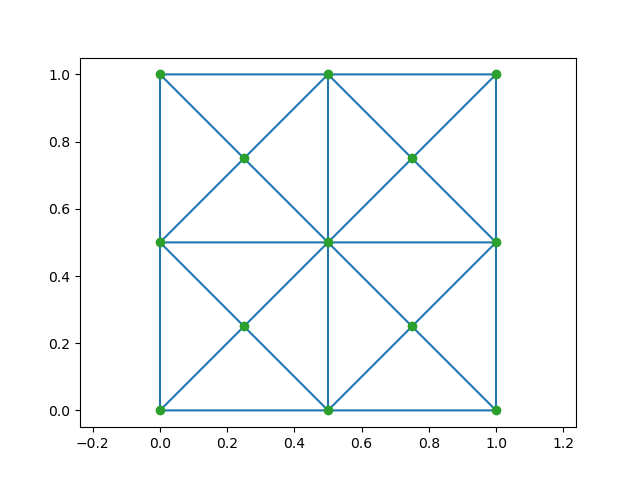
\includegraphics[width=0.9\linewidth]{./pics/final/pq30a0_1e.png}  
        \caption{角度不小于30,面积0.1}  
    \end{subfigure}%  
    \begin{subfigure}{0.5\textwidth}  
        \centering  
        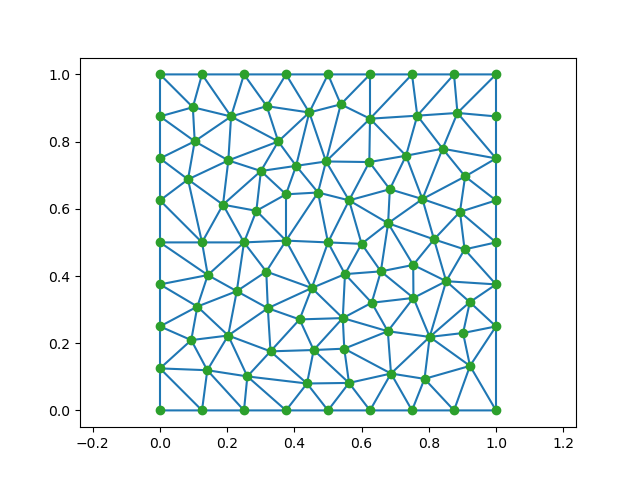
\includegraphics[width=0.9\linewidth]{./pics/final/pq30a0_01e.png}  
        \caption{角度不小于30,面积0.01}
    \end{subfigure}  
    \caption{SIPG}  

    \begin{subfigure}{0.5\textwidth}  
        \centering  
        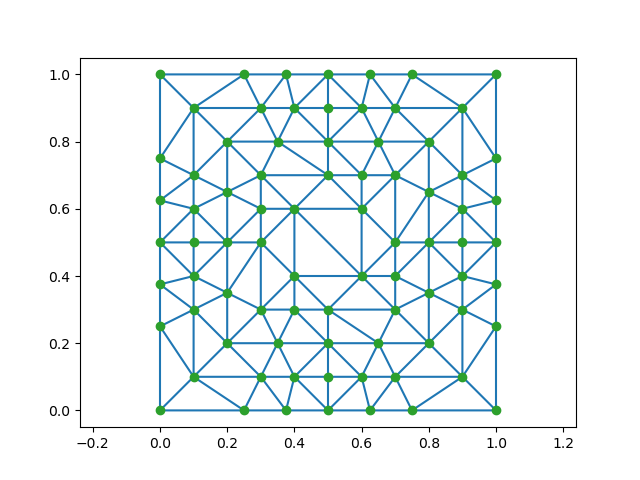
\includegraphics[width=0.9\linewidth]{./pics/final/spq30a0_1e.png}  
        \caption{内部设置强制边界,角度不小于30,面积0.1}  
    \end{subfigure}%  
    \begin{subfigure}{0.5\textwidth}  
        \centering  
        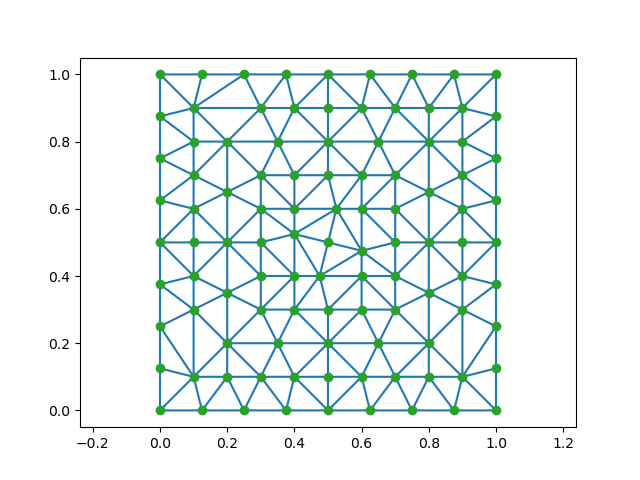
\includegraphics[width=0.9\linewidth]{./pics/final/spq30a0_01e.png}  
        \caption{内部设置强制边界,角度不小于30,面积0.01}
    \end{subfigure}  
    \caption{Triangle}  
\end{figure} 

\subsection*{代码}
相关代码上传到\url{https://gitee.com/Zebrainy-cgy/dgnet.git}


